% =====================================================================
%  Chapter 14 — The \idxw{Tail} at 4.77 Sigma
% =====================================================================

\chapter{The Tail at 4.77 Sigma}
\label{ch:tail}

The physical terms and the astrometric terms do not compete on equal
footing, and the reason is not the length of the arc. It is where the
keyhole sits in the distribution. A keyhole at the peak of the along-track\idx{Along-track}
distribution is insensitive to everything; a keyhole four and three-quarter
standard deviations out in the tail\idx{Tail} magnifies every error it is exposed to,
including the errors in the physics.

This chapter puts the two regimes side by side and computes the crossover.

\section{Regime one: a close encounter at seven years}

The 2024~YR4 lunar encounter of 22 December 2032 is the best-documented
near-term case, and the NASA review of the 2024~YR4 episode reports the
\idxw{B-plane} uncertainty for it with unusual clarity. The uncertainty was 270,000
kilometres, and the review records that a single point observation --- from
the Lucy spacecraft had it been available --- could have reduced it to
25,000 kilometres or less. The same review notes that the Lucy team's own
preliminary analysis did not regard this as certain, and that ground-based
observatories would be likely to achieve the same reduction by the end of the
apparition without Lucy.

That last clause is the important one. It means that the astrometric
uncertainty in a close-approach encounter is \emph{cheap} to reduce, and
that the community reduces it routinely.

Now put the physical term on the other side of the ledger. Over the seven
years from 2025 to 2032, an error in the Yarkovsky drift rate produces an
along-track\idx{Along-track} displacement of the object. The book's generator computes it
directly from the published drift-rate error, for a range of assumed drift
rates at a semimajor axis of 1.1 astronomical units.

\begin{table}[!htbp]
\centering
\small
\caption{Along-track displacement over seven years from an error in the
Yarkovsky drift rate, against the astrometric floor for the 2032 encounter.}
\label{tab:along-track}
\begin{tabularx}{\textwidth}{@{}P{1.07in}P{0.82in}P{0.82in}Y@{}}
\toprule
\rowcolor{panel}
\textbf{Drift rate} & \textbf{10 per cent} & \textbf{30 per cent} &
\textbf{Comment} \\
\midrule
50 m/yr & 0.3 km & 0.9 km & a slow drift \\
\rowcolor{panel}
100 m/yr & 0.6 km & 1.7 km & \\
300 m/yr & 1.7 km & 5.1 km & \\
\rowcolor{panel}
1,000 m/yr & 5.7 km & 17.2 km & the fastest case tabulated \\
\midrule
Astrometric floor & 25,000 km & 25,000 km & after a single observation \\
\bottomrule
\end{tabularx}
\end{table}

The comparison in \tabref{tab:along-track} is decisive at this horizon. Even
in the fastest case tabulated, a thirty per cent error in the drift rate
moves the object by 17.2 kilometres over seven years, against an astrometric
uncertainty of 25,000 kilometres after a single extra observation. The
astrometric term dominates by more than three orders of magnitude.

\begin{figure}[!htbp]
\centering
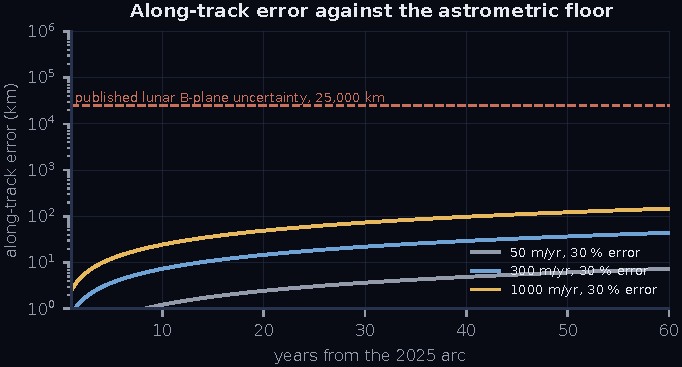
\includegraphics[width=\textwidth]{../figures/fig_along_track.pdf}
\caption{Along-track error against the length of the arc, for three assumed
drift rates and a thirty per cent rate error, against the published
astrometric floor of 25,000 kilometres. The two lines cross nowhere on this
axis: the astrometric term dominates at every horizon the 2032 encounter
reaches.}
\label{fig:along-track}
\end{figure}

The conclusion for this horizon is not that characterisation is useless. It
is that characterisation \emph{does not shorten this particular clock}. A
lunar station would not have made the 2032 lunar encounter probability
better, because the number that dominates that probability is the astrometric
uncertainty, and the astrometric uncertainty is cheap to reduce. That is a
statement about the seven-year horizon, and it is the reason the book's
selection rule declines the lunar platform for short-horizon objects.

\section{Regime two: a keyhole in the tail}

The 2036 encounter of Apophis is the other regime, and the difference is not
the horizon. It is the position of the keyhole.

The along-track\idx{Along-track} distribution for the 2036 encounter has a standard deviation
of 398.5 kilometres, as Chapter 11 reconstructed from the published keyhole
width and probability. The keyhole centre sits 4.77 standard deviations out
in the tail. In that regime the published sensitivity table's factors
translate into along-track displacements, because a probability ratio \(F\) in
the tail\idx{Tail} corresponds to a shift of \(\ln(F)/4.77\) standard deviations.

\begin{table}[!htbp]
\centering
\small
\caption{The published 2036 sensitivities, expressed as along-track
displacements against the 398.5-kilometre astrometric standard deviation.}
\label{tab:magnification}
\begin{tabularx}{\textwidth}{@{}P{1.22in}P{0.66in}P{0.83in}Y@{}}
\toprule
\rowcolor{panel}
\textbf{Varied assumption} & \textbf{Probability} & \textbf{Displacement} &
\textbf{Against the astrometric sigma} \\
\midrule
Diameter 270 \(\pm\) 60 m & \(\times 433\) & 507 km & 1.27 sigma \\
\rowcolor{panel}
Density variance, \(\sigma_\rho^{2} = 0.6\) & \(\times 93\) & 379 km &
0.95 sigma \\
\(\mu_{d0} = 400\) & \(\times 2.25\) & 68 km & 0.17 sigma \\
\rowcolor{panel}
Astrometric standard deviation & --- & 399 km & 1.00 sigma \\
\bottomrule
\end{tabularx}
\end{table}

\tabref{tab:magnification} is the heart of the book's argument about
platform selection. The diameter assumption and the density assumption each
move the 2036 keyhole centre by about one astrometric standard deviation.
They are \emph{not} smaller terms. They are the same size as the astrometric
uncertainty, and they point in a different direction.

\begin{seamnote}{The asymmetry that decides the rule}
Additional astrometry reduces the astrometric standard deviation, and it
reduces it monotonically: more observations, a longer arc, a better
reduction. Additional astrometry does nothing whatever to the 507 kilometres
of displacement contributed by the diameter assumption, or the 379
kilometres contributed by the density, because those are not astrometric
quantities. A rule that selects a platform on the basis of the astrometric
term alone will always choose the ground. A rule that includes the physical
term does not.
\end{seamnote}

\section{The crossover, stated as a principle}

The two regimes are not separated by the horizon and they are not separated
by the instrument. They are separated by whether the keyhole lies in the
tail\idx{Tail} of the along-track distribution.

Where the keyhole is near the peak, the probability is set by the
astrometric uncertainty, the astrometric uncertainty is cheap to reduce, and
characterisation buys nothing. This is the 2032 lunar encounter of
2024~YR4, where a thirty per cent drift-rate error is worth 17 kilometres
against an astrometric floor of 25,000.

Where the keyhole lies several sigma out, the physical terms are of the same
order as the astrometric term and they do not shrink with observing time.
This is the 2036 encounter of Apophis, where the diameter assumption alone is
worth 507 kilometres of displacement.

\begin{table}[!htbp]
\centering
\small
\caption{The two regimes, and what each one implies for a platform.}
\label{tab:regimes}
\begin{tabularx}{\textwidth}{@{}P{1.28in}P{1.28in}Y@{}}
\toprule
\rowcolor{panel}
\textbf{Regime} & \textbf{Dominated by} & \textbf{Implication} \\
\midrule
Keyhole near the peak & astrometry & observe more; the ground does this
best \\
\rowcolor{panel}
Keyhole several sigma out & physics, comparably & measure the size and the
density \\
\bottomrule
\end{tabularx}
\end{table}

This is why the platform-selection rule in Chapter 30 has a conditional
clause at its centre, and why the lunar platform is proposed for a class of
targets rather than for a class of instruments. The lunar station does not
help with the astrometric term. It helps with the physical term. It is worth
exactly as much as the physical term is worth, and the physical term is
worth a great deal when the keyhole is in the tail.

\begin{keytakeaways}
\item At the 2032 lunar encounter of 2024 YR4, a thirty per cent drift-rate
error is worth 17.2 kilometres against an astrometric floor of 25,000 after
a single observation, and the astrometric term dominates by three orders of
magnitude.
\item At the 2036 encounter of Apophis, the diameter assumption alone is
worth 507 kilometres of keyhole displacement and the density assumption 379
kilometres, against an astrometric standard deviation of 399 kilometres.
\item The two regimes are separated by the position of the keyhole in the
tail, not by the length of the arc.
\item More astrometry shrinks the astrometric term and does nothing to the
physical one, which is the asymmetry the selection rule turns on.
\end{keytakeaways}
